\documentclass[aspectratio=169]{beamer} % Proporção 16:9 para telas modernas

% --- Pacotes e Configurações de Cores ---
\usepackage[utf8]{inputenc}
\usepackage[T1]{fontenc}
\usepackage{graphicx}
\usepackage{booktabs}
\usepackage{amsmath, amsfonts, amssymb}
\usepackage{tikz}
\usepackage{pgfplots}
\pgfplotsset{compat=1.18}

% Paleta de Cores Inovadora (Dark Mode)
\definecolor{DeepBlack}{HTML}{0B0E14}
\definecolor{AccentCyan}{HTML}{00F2FF}
\definecolor{MutedGray}{HTML}{2D3436}
\definecolor{TextWhite}{HTML}{F0F0F0}
\definecolor{SoftRed}{HTML}{FF4757}

% --- Configurações do Beamer ---
\setbeamercolor{background canvas}{bg=DeepBlack}
\setbeamercolor{normal text}{fg=TextWhite}
\setbeamercolor{frametitle}{fg=AccentCyan}
\setbeamercolor{title}{fg=AccentCyan}
\setbeamercolor{section in toc}{fg=TextWhite}
\setbeamercolor{block title}{fg=DeepBlack, bg=AccentCyan}
\setbeamercolor{block body}{fg=TextWhite, bg=MutedGray}
\setbeamercolor{item}{fg=AccentCyan}

% Removendo botões de navegação feios
\setbeamertemplate{navigation symbols}{}

% Design do Frame Title Customizado
\setbeamertemplate{frametitle}{
    \vspace{0.3cm}
    \begin{minipage}{0.9\textwidth}
        \flushleft
        \insertframetitle \\
        \tikz \draw[AccentCyan, line width=1pt] (0,0) -- (2,0); % Linha minimalista
    \end{minipage}
}

% Design dos Rodapés
\setbeamertemplate{footline}{
    \hfill
    \tikz \node[TextWhite, opacity=0.3] at (0,0) {\small \insertframenumber / \inserttotalframenumber};
    \hspace{0.5cm} \vspace{0.3cm}
}

% --- Início do Documento ---
\title{Apresentação de Teste}
\subtitle{Exemplo Completo em \LaTeX}
\author{Autor Exemplo}
\institute{Instituição Exemplo}
\date{\today}

\begin{document}

% Slide 1 - Capa (Design de Impacto)
{
\setbeamertemplate{footline}{} % Remove rodapé da capa
\begin{frame}
    \centering
    \begin{tikzpicture}[remember picture, overlay]
        \fill[MutedGray] (current page.north west) rectangle ([xshift=0.5cm]current page.south west);
        \draw[AccentCyan, line width=2pt] ([xshift=0.6cm]current page.north west) -- ([xshift=0.6cm]current page.south west);
    \end{tikzpicture}
    
    {\Huge \textbf{\inserttitle}} \\
    \vspace{0.2cm}
    {\large \color{AccentCyan} \insertsubtitle} \\
    \vspace{1.5cm}
    \textbf{\insertauthor} \\
    \textit{\small \insertinstitute} \\
    \vspace{0.5cm}
    \small \insertdate
\end{frame}
}

% Slide 2 - Sumário
\begin{frame}{Sumário}
    \tableofcontents
\end{frame}

% Slide 3 - Introdução
\section{Introdução}
\begin{frame}{Introdução}
    Esta é uma apresentação de teste criada em \LaTeX\ utilizando o pacote \textbf{Beamer}.
    \vspace{0.5cm}
    \begin{quote}
        O objetivo é demonstrar diversos recursos comuns em apresentações acadêmicas com um visual disruptivo.
    \end{quote}
\end{frame}

% Slide 4 - Texto e Parágrafo
\begin{frame}{Texto e Parágrafo}
    O \LaTeX\ é amplamente utilizado para produção de documentos científicos, 
    pois oferece alta qualidade tipográfica.

    \vspace{0.8cm}
    \begin{columns}
        \column{0.5\textwidth}
        \textbf{Controle Total} \\
        Excelente controle de formatação e precisão em cada caractere.
        
        \column{0.5\textwidth}
        \textbf{Versatilidade} \\
        Indicado para fórmulas matemáticas, tabelas e referências automáticas.
    \end{columns}
\end{frame}

% Slide 5 - Lista Simples
\begin{frame}{Lista Simples}
    \begin{itemize}
        \item Alta qualidade tipográfica
        \item Organização estrutural
        \item Facilidade com matemática
        \item Uso acadêmico e profissional
    \end{itemize}
\end{frame}

% Slide 7 - Matemática (Visual Limpo)
\section{Matemática}
\begin{frame}{Fórmula Matemática}
    \centering
    A famosa equação da relatividade é dada por:
    \vspace{0.5cm}
    {\huge \color{AccentCyan} $$E = mc^2$$}
    \vspace{0.5cm}
    \small onde $E$ é a energia, $m$ a massa e $c$ a velocidade da luz.
\end{frame}

% Slide 9 - Bloco de Destaque (Design Flat)
\begin{frame}{Bloco de Informação}
    \begin{block}{Definição}
        Uma função é uma relação que associa cada elemento de um conjunto 
        a exatamente um elemento de outro conjunto.
    \end{block}
\end{frame}

% Slide 11 - Tabelas (Minimalistas)
\section{Tabelas}
\begin{frame}{Tabela Simples}
    \centering
    \begin{table}
        \color{TextWhite}
        \begin{tabular}{l c c}
            \toprule
            \textbf{\color{AccentCyan} Item} & \textbf{\color{AccentCyan} Valor A} & \textbf{\color{AccentCyan} Valor B} \\
            \midrule
            A & 10 & 20 \\
            B & 15 & 25 \\
            C & 30 & 40 \\
            \bottomrule
        \end{tabular}
        \caption{\color{TextWhite} Exemplo de tabela clean}
    \end{table}
\end{frame}

% Slide 13 - Gráfico (Estilo Dark)
\section{Gráficos}
\begin{frame}{Gráfico de Barras}
\centering
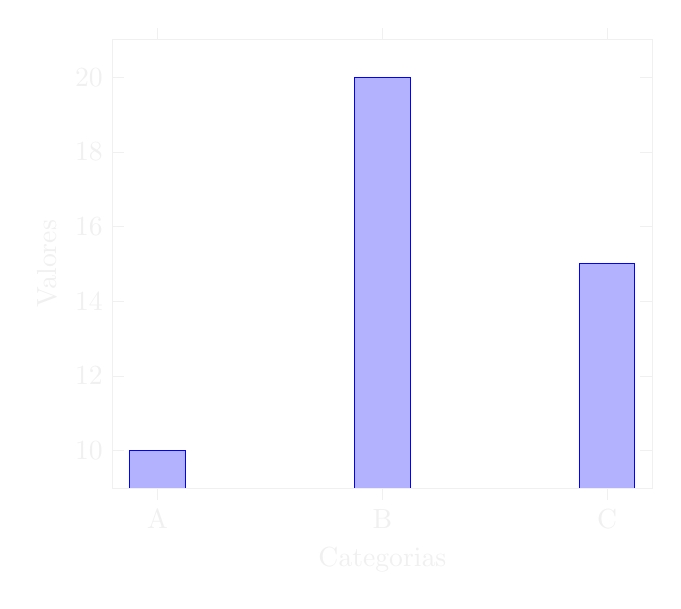
\begin{tikzpicture}
\begin{axis}[
    ybar,
    axis line style={TextWhite},
    tick style={TextWhite},
    label style={TextWhite},
    tick label style={TextWhite},
    xlabel={Categorias},
    ylabel={Valores},
    symbolic x coords={A,B,C},
    xtick=data,
    bar width=20pt,
    fill=AccentCyan,
    draw=AccentCyan,
    area style
]
\addplot coordinates {(A,10) (B,20) (C,15)};
\end{axis}
\end{tikzpicture}
\end{frame}

% Slide 16 - Alerta
\begin{frame}{Alerta}
    \setbeamercolor{block title}{bg=SoftRed, fg=DeepBlack}
    \begin{block}{Atenção}
        Sempre revise a estrutura e a coerência da sua apresentação.
    \end{block}
\end{frame}

% Slide 20 - Encerramento
\begin{frame}
    \centering
    
\begin{tikzpicture}
        \draw[AccentCyan, line width=2pt] (0,0) circle (1.5cm);
        \node at (0,0) {\Huge \textbf{?}};
    \end{tikzpicture}
    \vspace{0.5cm}
    {\Huge \textbf{\color{AccentCyan} Obrigado!}} \\
    \vspace{0.3cm}
    Perguntas?
\end{frame}

\end{document}